% http://www.ctan.org/tex-archive/macros/latex/contrib/beamer/examples
% http://latex.artikel-namsu.de/english/beamer-examples.html

\documentclass{beamer}
\usepackage{amsmath}
\usepackage{amssymb}
\usepackage{bm}
\usepackage{fancybox, graphicx}
\usepackage{listings}


\lstdefinestyle{customc}{
  belowcaptionskip=1\baselineskip,
  breaklines=true,
  %frame=L,
  xleftmargin=\parindent,
  language=bash,
  showstringspaces=false,
  basicstyle=\footnotesize\ttfamily,
  keywordstyle=\bfseries\color{green!40!black},
  commentstyle=\itshape\color{purple!40!black},
  identifierstyle=\color{blue},
  stringstyle=\color{orange},
}

\lstset{style=customc}

\usetheme{Dresden}


\title[HPC Workshop] % (optional, use only with long paper titles)
{HPC Workshop}

\author[Balan,Palmese,Saadeh] % (optional, use only with lots of authors)
{S.~T.~Balan, A.~Palmese,D.~Saadeh}

\institute[UCL]
{
  Department of Physics and Astronomy\\
  University College London
}
\date[HPC 2015]
{22 October 2015}

\subject{HPC}

\begin{document}

\frame{\titlepage}

\section{Basics}

\begin{frame}{Information on the Web}
  \begin{block}{This presentation}
    \url{https://github.com/Astrophysics-UCL/HPCInfo/}
  \end{block}

    \begin{block}{Splinter on the UCL Astrophysics Wiki}
    \url{https://wiki.ucl.ac.uk/display/PhysAstAstPhysGrp/Splinter+User+Guide}
  \end{block}

  \begin{block}{UCL Research Computing Platforms}
    \url{https://wiki.rc.ucl.ac.uk/wiki/Main_Page}
  \end{block}

  \begin{block}{DiRAC}
    \url{http://www.dirac.ac.uk/}
  \end{block}

\end{frame}

\begin{frame}{Mailing list}
	\url{https://www.mailinglists.ucl.ac.uk/mailman/listinfo/splinter-users}
	\bigskip
	\begin{itemize}
		\item please subscirbe
		\item post any issues regarding splinter
	\end{itemize}
\end{frame}

\begin{frame}{What will you learn?}
  \begin{itemize}
    \item Running your programs in HPC machines
	\item Best practices
  \end{itemize}
\end{frame}


\begin{frame}{Splinter specs}
	\begin{itemize}
		\item As of \today, \emph{Splinter} has 528, 4TB memory
		\item 8 nodes, dual 6-core 2.8GHz, 48GB memory 
		\item 20 nodes, dual 8-core 2.0GHz, 128GB memory
		\item SMP node, 40 2.4GHz cores, 1TB memory
		\item login node, dual 10-core, 2.4GHz 98GB memory
		\item head-node, dual 8-core, 2.4GHz, 164GB memory
	\end{itemize}
\end{frame}

\begin{frame}{\textsc{splinter} distributed}
  \begin{figure}
    \begin{center}
      \shadowbox{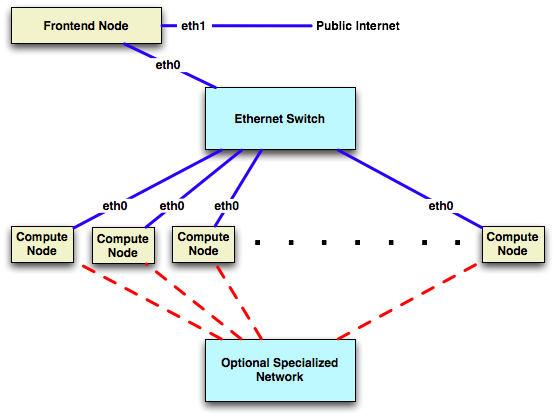
\includegraphics[scale=0.4]{cluster.png}}
      \footnote{\url{http://www.rocksclusters.org/}}
    \end{center}
  \end{figure}
\end{frame}

\begin{frame}{\textsc{splinter} shared}
  \begin{figure}
    \begin{center}
      \shadowbox{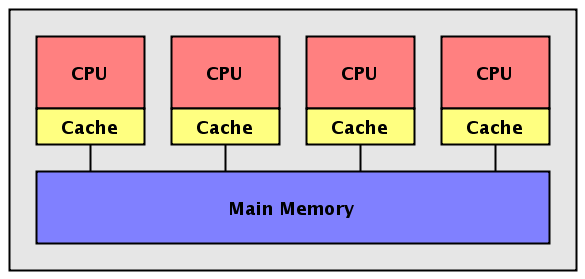
\includegraphics[scale=0.4]{fig03.png}}
      \footnote{\url{http://www.cs.rit.edu/}}
    \end{center}
  \end{figure}
\end{frame}

\begin{frame}{Workspaces I}
	\begin{block}{\texttt{/home/user\_name}}
		\begin{itemize}
			\item this is your home directory
			\item login scripts can be put here
			\item 1GB quota
			\item private
		\end{itemize}
	\end{block}
	\begin{block}{\texttt{/share/splinter/user\_name}}
		\begin{itemize}
			\item create the directory if not already there
			\item can be used as a workspace
			\item no quota
			\item public unless made private
		\end{itemize}
	\end{block}
\end{frame}

\begin{frame}{Workspaces II}
	\begin{block}{\texttt{/share/data1}}
		\begin{itemize}
			\item for storing large data
			\item you can create a directory for your, .e.g, \texttt{/share/data1/SKA}
		\end{itemize}
	\end{block}

	\begin{block}{\texttt{/share/apps}}
		\begin{itemize}
			\item for installing software
			\item module-files
		\end{itemize}
	\end{block}
\end{frame}

\begin{frame}[fragile]{Login script}
	\begin{itemize}
		\item everytime you login this file will be executed
		\item this file is in your \texttt{\$HOME}
		\item it is called \texttt{.login}
		\item you can load modules, envvars, etc.
	\end{itemize}
	\begin{block}{example}
		\lstinputlisting{dot_login.sh}
	\end{block}
\end{frame}

\begin{frame}[fragile]{Modules}
	\begin{itemize}
		\item easy and flexible way use software
		\item available to everyone in splinter
	\end{itemize}

	\begin{block}{commands}
		\lstinputlisting{modules.sh}
	\end{block}
\end{frame}

\begin{frame}[fragile]{Submitting jobs}
	\begin{itemize}
		\item computing jobs should be submitted to the scheudler
		\item you will have to write a job script
		\item interactive job
	\end{itemize}
    \begin{block}{commands}
      \lstinputlisting{job_submission.sh}
    \end{block}
\end{frame}

\begin{frame}{Queues}
	\begin{itemize}
		\item \texttt{compute}
		\item \texttt{cores16}
		\item \texttt{cores12}
		\item \texttt{smp}
	\end{itemize}
\end{frame}

\begin{frame}[fragile]{Structure of a job script}
	\lstinputlisting{sample_job_script.sh}
\end{frame}

\begin{frame}{Jobscripts: things to remember}
	\begin{itemize}
		\item Submit the job to the right queue
		\item Request the correct number of \texttt{nodes} and \texttt{ppn}
		\item Specify the memory required
		\item Always specify the walltime
		\item If your program is not parallel, please use \texttt{nodes=1,ppn=1}
		\item Use \texttt{-q compute} for single processor jobs
		\item Use \texttt{qsub -I} for interative job
		\item If using most of the resources, please send an email to the mailing list.
	\end{itemize}
\end{frame}

\begin{frame}[fragile]{More PBS commands}
	\lstinputlisting{pbs_extra_commands.sh}
\end{frame}

\begin{frame}{Using \emph{Gaglia}}
	\url{http://splinter.star.ucl.ac.uk/ganglia/}

	\begin{itemize}
		\item is tool for analysing splinter
		\item can only be loaded from splinter (using firefox)
		\item will give you load/memory information
		\item can look into nodes
	\end{itemize}
\end{frame}

\begin{frame}{Collaborative projects}
	\begin{itemize}
		\item collaboration between two splinter users
		\item can share common data in \texttt{/share/data1/my\_collaboration}
		\item give read/write permission to other users using \texttt{chmod}
	\end{itemize}
\end{frame}


\begin{frame}{Best practices}
  \begin{itemize}
    \item Choose the machines that are suited for your problem
    \item Read the User Guide
    \item Do not run your programs in the login node
    \item Install common software locally if and only if absolutely necessary
    \item Request optimum resouces
    \item Minimise data transfer between nodes,
    \item \alert{Backup! Backup! Backup!}
  \end{itemize}
\end{frame}

\begin{frame}{Exercises}
	\url{https://github.com/Astrophysics-UCL/HPCInfo/blob/master/training/workshops_2015/hpc_workshop/exercies/exercises.md}
\end{frame}


\end{document}
